\chapter{Introduction}\label{ch:intro}

\section{The question}

A defender protects a set of targets with a few identical resources, say patrol units. She cannot cover
every target, so she randomizes. An attacker picks one target to attack. The attacker comes in several
\emph{types}, drawn from a known prior; each type values the targets differently, and only the attacker
knows his type. Both move at the same time. An attack on a covered target is no better for the attacker and
no worse for the defender than an attack on an uncovered one. This is a \emph{Bayesian simple security
game}.

A \emph{Bayes--Nash equilibrium} (BNE) is a mixed strategy for the defender and one for every attacker
type such that nobody can gain by deviating. Nash's theorem says that one exists. Conitzer's question
is whether one can be \emph{computed} in time polynomial in the size of the explicitly listed
payoff tables~\cite{conitzer26}. The question has been open since 2015.

\section{A small example}\label{sec:intro-example}

Take two targets, one defender resource and two attacker types. The defender gets $0$ when an attacked
target is uncovered and $1$ when it is covered. Write $x_1$ for the probability that target~$1$ is
covered; then target~$2$ is covered with probability $x_2=1-x_1$.
\begin{itemize}[nosep]
\item Type~1 has prior $2/3$. It gets $3/2$ at target~$1$ if uncovered and $1/2$ if covered, and $1$ at
target~$2$ if uncovered and $0$ if covered. Its expected payoffs are $3/2-x_1$ and $1-x_2=x_1$.
\item Type~2 has prior $1/3$. It gets $1-x_1$ at target~$1$ and $-x_2$ at target~$2$.
\end{itemize}
Type~2 prefers target~$1$ whenever $x_1<1$, since $1-x_1>x_1-1$. The defender's payoff is the
probability that the attacked target is covered, so she wants to cover the target that is attacked
more often.

Can the defender cover both targets with positive probability? Only if she is indifferent, that is, if
both targets are attacked with the same total probability $1/2$. Type~2 sends $1/3$ to target~$1$, so
type~1 must send $1/6$ to target~$1$ and $1/2$ to target~$2$. Type~1 mixes only if it is indifferent:
$3/2-x_1=x_1$, so $x_1=3/4$. This gives the equilibrium
\[
x=(3/4,\,1/4),\qquad \text{type 1 attacks }(1/4,\,3/4),\qquad \text{type 2 attacks target }1.
\]
(No other coverage works: if $x_1>3/4$, type~1 attacks only target~2, which then carries load at least $2/3$, and
the defender would move all coverage there; if $x_1<3/4$, every attack goes to target~1.)
Figure~\ref{fig:example-market} draws this equilibrium.

\begin{figure}[t]
\centering
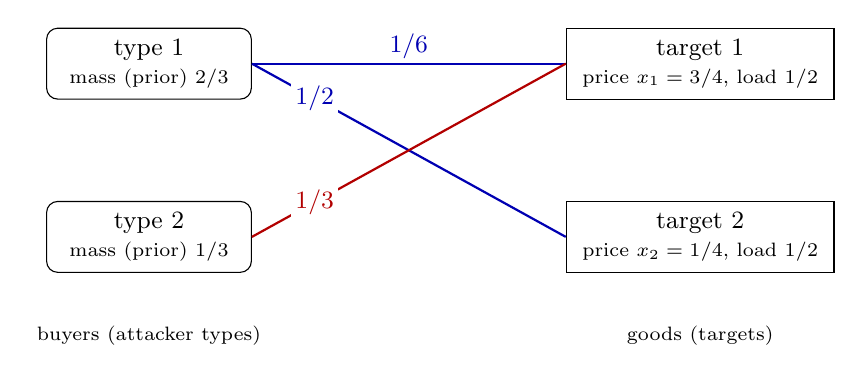
\begin{tikzpicture}[
  ty/.style={draw,rounded corners,minimum width=2.6cm,minimum height=0.9cm,align=center,font=\small},
  tg/.style={draw,minimum width=3.4cm,minimum height=0.9cm,align=center,font=\small},
  lb/.style={font=\small,fill=white,inner sep=1.5pt}]
  \node[ty] (t1) at (0,1.1) {type 1\\[-1pt]{\scriptsize mass (prior) $2/3$}};
  \node[ty] (t2) at (0,-1.1) {type 2\\[-1pt]{\scriptsize mass (prior) $1/3$}};
  \node[tg] (g1) at (7,1.1) {target 1\\[-1pt]{\scriptsize price $x_1=3/4$, load $1/2$}};
  \node[tg] (g2) at (7,-1.1) {target 2\\[-1pt]{\scriptsize price $x_2=1/4$, load $1/2$}};
  \draw[thick,blue!70!black] (t1.east) -- node[lb,pos=0.5,above]{$1/6$} (g1.west);
  \draw[thick,blue!70!black] (t1.east) -- node[lb,pos=0.2]{$1/2$} (g2.west);
  \draw[thick,red!70!black] (t2.east) -- node[lb,pos=0.2]{$1/3$} (g1.west);
  \node[font=\scriptsize,align=center] at (0,-2.35) {buyers (attacker types)};
  \node[font=\scriptsize,align=center] at (7,-2.35) {goods (targets)};
\end{tikzpicture}
\caption{The example of Section~\ref{sec:intro-example} read as a market. Edges carry the equilibrium
attack masses $f_{ij}$; each type's edges sum to its prior. The coverage $x$ acts as the price vector.
Type~1 uses both targets and is indifferent there ($3/2-x_1=1-x_2=3/4$); type~2 uses only
target~1. Both targets are partly covered, so the defender must be indifferent, and indeed both loads
equal the common level $1/2$, which plays the role of the capacity $\lambda/d_j$ with cutoff
$\lambda=1/2$ and $d_j=1$ (Lemma~\ref{lem:mk-box-cutoff}).}
\label{fig:example-market}
\end{figure}

The example shows the two forces of every equilibrium. The \emph{coverage} makes the attackers
indifferent, and the \emph{attack loads} make the defender indifferent. Read coverage as a price and
attack load as demand: target~$j$ is a good, each type is a buyer with a mass equal to its prior,
covering a target makes it ``more expensive'' to attack, and the defender adjusts the prices until the
demand for each partly covered good equals a common level (here $1/2$). This market reading is the
starting point of the whole book (Chapter~\ref{ch:market}).

\section{Why the question is hard to settle}

When every attacker slope $u^0-u^1$ equals one, or more generally when the slopes factor into a type
part times a target part, the market's equilibrium conditions are the optimality conditions of one
linear program (Section~\ref{sec:ar-gadget-market}). In general the slopes differ from type to type
and from target to target. Then the equilibrium conditions are a
genuine fixed-point problem: the set of targets each type uses and the set of targets the defender
covers are combinatorial choices, and the right choice is not known in advance. The equilibria need not
be unique, and averaging two ordered equilibria of the fixed-cutoff market does not give an
equilibrium of the game (Example~\ref{ex:mk-interp}). On the other hand, the problem has much structure: payoffs are affine in
the coverage, and the defender's best response is a fractional knapsack.

The results of this book place the problem between two known landmarks. From below it is at least as
hard as ARRIVAL, a zero-player game whose complexity is itself open. From above it lies in
$\mathsf{UEOPL}$, a class of total search problems that is also the best known class upper bound for
ARRIVAL.
Figure~\ref{fig:landscape} shows the picture.

\begin{figure}[t]
\centering
\begin{tikzpicture}[
  box/.style={draw,rounded corners,minimum width=2.3cm,minimum height=0.8cm,align=center,font=\small},
  cls/.style={draw,dashed,rounded corners,minimum width=2.0cm,minimum height=0.7cm,align=center,font=\small},
  arr/.style={-{Stealth[length=2.5mm]},thick},
  lab/.style={font=\scriptsize,midway,fill=white,inner sep=1.5pt}]
  \node[box] (arr) at (-1.0,0) {ARRIVAL};
  \node[box] (bne) at (4.2,0) {exact BNE};
  \node[box] (m1)  at (8.4,0) {(M1) market};
  \node[box] (plcp) at (8.4,-2.6) {P-LCP};
  \node[cls] (ueopl) at (4.2,-4.6) {$\mathsf{UEOPL}$};
  \node[cls] (eopl) at (4.2,-5.9) {$\mathsf{EOPL}=\mathsf{CLS}$};
  \draw[arr,vlean,line width=1.6pt] (arr) -- node[lab,align=center]{$\le_m$ (Ch.~\ref{ch:arrival};\\ Lean: App.~\ref{app:short})} (bne);
  \draw[arr,vref,{Stealth[length=2.5mm]}-{Stealth[length=2.5mm]}] (bne) -- node[lab]{$\equiv_T$ (Ch.~\ref{ch:market})} (m1);
  \draw[arr,vpartial,line width=1.3pt,dashed] (m1) -- node[lab]{$\le_m$ (Ch.~\ref{ch:upper})} (plcp);
  \draw[arr,vpartial,line width=1.3pt,dashed] (bne) -- node[lab,pos=0.55]{$\le_m$, direct (Ch.~\ref{ch:upper})} (plcp);
  \draw[arr,vref] (arr.north) |- node[lab,pos=0.75]{ARRIVAL $\le_m$ P-LCP, new (Cor.~\ref{plcp:cor:arrival})} (10.3,1.1) |- (plcp.east);
  \draw[arr,vpartial,line width=1.3pt,dashed] (bne) -- node[lab,pos=0.45]{$\in$, one $\ell_1$ contraction (Ch.~\ref{ch:upper})} (ueopl);
  \draw[arr,gray] (plcp) to[out=-90,in=0] node[lab,pos=0.4]{$\in$ \cite{fgms18}} (ueopl);
  \draw[arr,gray] (arr) to[out=-90,in=180] node[lab,pos=0.6]{$\in$ \cite{ghhkms18,fgms18}} (ueopl);
  \draw[arr,gray] (ueopl) -- node[lab,right=2pt,fill=none]{$\subseteq$} (eopl);
  \node[draw,align=left,font=\small,anchor=north west] at (-1.2,-6.7) {%
    \textbf{Algorithms for exact BNE} ($n$ targets, $m$ types, input length $L$):\\
    $\bullet$ $L^{O(\sqrt n)}$ bit operations (Ch.~\ref{ch:upper}, after Ghorbani--Lopes--Mnich);\\
    $\bullet$ $L^{O(\sqrt{\min(m,n)})}$ via the game-to-market reduction (Prop.~\ref{prop:sx-min});\\
    $\bullet$ the Li--Conitzer--Korzhyk algorithm needs $\ge2^{h-1}$ steps on games $\Gamma_h$ (Ch.~\ref{ch:lck}).};
\end{tikzpicture}
\caption{The landscape. Arrow colors show how each arrow's correctness was checked: \textcolor{vlean}{\textbf{dark green, thick}} = correctness machine-checked in Lean (via the Appendix~\ref{app:short} construction; running time not formalized); \textcolor{vpartial}{\textbf{light green, dashed}} = partly machine-checked (Section~\ref{sec:lean-status} lists what is covered); \textcolor{vref}{\textbf{amber}} = checked by independent AI referees; gray = known results. $\mathsf{EOPL}=\mathsf{CLS}$ by~\cite{gjhmprt22,fghs23}. $\le_m$ is a polynomial-time many-one reduction, $\equiv_T$ polynomial-time Turing
equivalence. The top arrow composes ARRIVAL $\le_m$ (M1) (Theorem~\ref{thm:arrival-m1}) with (M1) $\le_m$ P-LCP (Theorem~\ref{plcp:thm:main}). The direct arrow from exact BNE to P-LCP is the reduction of Section~\ref{sec:direct-lcp}; it gives a second proof that exact BNE is in $\mathsf{UEOPL}$. Exact BNE refers to Bayesian simple security games (Definition~\ref{def:game}); in general Bayesian games, equilibrium search is already $\mathsf{PPAD}$-hard.}
\label{fig:landscape}
\end{figure}

\section{The ideas in plain words}\label{sec:intro-ideas}

This section says, without formulas, why the main results should be true. Each paragraph ends with
where the precise statement and its proof are.

\paragraph{The game is a market.} Read the defender's coverage of a target as its \emph{price}. An
attacker type goes to the target that is best for it, and a target gets less attractive the more it is
covered, just as a buyer goes to the good that is best at current prices, and a good gets less
attractive the more it costs. The defender puts coverage where the expected loss is highest, up to the
budget, just as a market raises the prices of goods that are in high demand. So an equilibrium of the
game is a set of prices at which every buyer is content with what it buys: an equilibrium of a matching
market (Chapter~\ref{ch:market}).

\paragraph{A market can imitate a train.} In ARRIVAL a token walks through switches, and each switch
sends it alternately to its two exits: the first visit goes one way, the second the other, the third the
first way again. If many visits are counted at once, a switch that is visited $x$ times sends about
half of them each way, with the extra one on the first exit. Allowing $x$ to be fractional turns this
rule into a continuous ``splitting'' rule, and every flow that splits consistently at every switch, even
a fractional one, still reveals where the token ends (Section~\ref{sec:pre-arrival},
Lemma~\ref{lem:decoder}). Chapter~\ref{ch:arrival} builds, for each switch, a small market whose
equilibria split the flow they receive by exactly this rule. The difficulty is that market equilibria
are smooth and look convex, while alternation is a parity effect. The trick is a network of Disser and
Skutella in which the cheapest way to send each further unit of flow costs more than the last. Two
copies of it share one source; whichever copy is currently cheaper takes the next unit, and the two
take turns, like a switch. Glued together along the graph, the gadgets give a market, and hence a game,
in which every equilibrium is a consistent splitting flow. An exact equilibrium therefore answers the
ARRIVAL instance (Chapter~\ref{ch:arrival}).

\paragraph{Why the problem is no harder than P-LCP.} Every equilibrium condition has the form ``either
this quantity is zero or that constraint is tight'': a type attacks a target only if the target is best
for it, a target is covered only if it draws enough attack, and the budget is used up. A system of such
conditions is a linear complementarity problem. Attacks and coverage are coupled through one table of
type--target pairs, read once from the attackers' side and once from the defender's. Because of this
mirror structure every principal minor of the problem's matrix is a product of two determinants of the
same sign, so none is negative. A tiny perturbation then makes every one positive: the matrix becomes a
P-matrix, the problem has exactly one solution, and one linear program turns the pattern of that solution
into an exact equilibrium. Problems with this kind of unique answer lie in $\mathsf{UEOPL}$
(Section~\ref{sec:direct-lcp}).

\paragraph{Why it can be solved in $L^{O(\sqrt n)}$.} The game can also be written as an update rule
that moves a candidate coverage toward the players' best responses, damped so that it brings any two
points closer together. Its unique fixed point is the equilibrium. For such a rule, evaluating it at one
point shows on which side of a hyperplane through that point the fixed point lies, so one can search by
repeated cutting, a binary search in many dimensions. Doing this in blocks of about $\sqrt n$ coordinates
with the deep-point method of Ghorbani, Lopes and Mnich gives the bound
(Sections~\ref{sec:contraction} and~\ref{sec:subexp}).

\paragraph{Why the published algorithm is slow.} Li, Conitzer and Korzhyk raise the defender's budget
from zero and follow the equilibrium as it moves; each step is a straight segment. Chapter~\ref{ch:lck}
builds games in which a small circuit of min and max gates folds the equilibrium path, like a strip of
paper folded in half again and again, so that the path has exponentially many bends. Any method that
follows it in straight segments needs exponentially many steps, even though the final equilibrium of
these particular games is easy to compute by other means (Proposition~\ref{artlck:prop:easy}).

\paragraph{Why the question stays open.} The two bounds meet ARRIVAL from both sides: from below the
problem is at least as hard as ARRIVAL, and from above it lies in $\mathsf{UEOPL}$, which is also the
best known upper bound for ARRIVAL. A polynomial-time algorithm would therefore also solve ARRIVAL,
which has resisted all attempts since it was introduced~\cite{dgkmw17}.

\section{What each chapter does}

\paragraph{Chapter~\ref{ch:prelim}: Preliminaries.} All definitions in one place: the game, coverage
vectors and the cutoff form of equilibrium, the affine matching market (M1), ARRIVAL and its continuous
switch map, reductions, and the complexity classes.

\paragraph{Chapter~\ref{ch:market}: The game is a market.} Exact BNE search and exact equilibrium search
in (M1) are polynomial-time Turing equivalent. From market to game one oracle call suffices, and the
game produced has one resource, defender payoffs $0$ and $1$ and nearly uniform priors; so these
restricted games are already as hard as the general ones. From game to market the reduction bisects over
the defender's cutoff and repairs the budget exactly by linear programming.

\paragraph{Chapter~\ref{ch:arrival}: ARRIVAL-hardness.} An ARRIVAL instance with $n$ switches becomes a
one-resource game with at most $12n^2+6n+6$ types, and every BNE reveals the answer. Each switch is
simulated by a small market gadget built from two offset copies of the Disser--Skutella counting
network, whose cheapest flows alternate between the two copies exactly like a switch.

\paragraph{Chapter~\ref{ch:upper}: Upper bounds.} The market's equilibrium conditions are a linear
complementarity problem with a $P_0$ matrix; a tiny diagonal perturbation makes it a P-matrix, so (M1)
and ARRIVAL reduce many-one to P-LCP. Separately, the game itself is encoded as the unique fixed point
of one explicit piecewise-linear $\ell_1$ contraction. Read as a PL-Contraction instance this puts exact
BNE in $\mathsf{UEOPL}$; fed to the block search of Ghorbani, Lopes and Mnich it gives an
$L^{O(\sqrt n)}$ algorithm.

\paragraph{Chapter~\ref{ch:lck}: An exponential lower bound for the Li--Conitzer--Korzhyk algorithm.} That algorithm raises
the defender's budget continuously and follows equilibria along straight segments. A folding circuit of
min and max gates produces a game whose equilibrium path is unique for budgets up to $3/8$ and has $2^{h-1}$ affine pieces there, so the algorithm
needs at least $2^{h-1}$ segments. A second family forces $2^n$ distinct attack patterns.

\paragraph{Chapter~\ref{ch:open}: Open problems.} What the results do not show.

\section{What remains open}

The main question remains open: polynomial time is neither proved nor ruled out. The lower bound
matters only if ARRIVAL is not in $\mathsf P$, and the upper bound does not give a polynomial algorithm.
It is not known whether exact BNE is $\mathsf{UEOPL}$-hard, whether it reduces to ARRIVAL, or whether
P-LCP reduces back to the market. Chapter~\ref{ch:open} lists these and smaller questions.
